\documentclass{beamer}
\usecolortheme{dove}
\setbeamertemplate{navigation symbols}{}
\setbeamertemplate{footline}[text line]{\parbox{\linewidth}{\vspace*{-8pt}\insertsectionnavigationhorizontal{.97\paperwidth}{\hspace{-32pt}}{\hfill\hfill}}}
\usepackage{amsmath,amssymb,amsfonts,amsthm, multicol, subfigure, color}
\usepackage{bm}
\usepackage{graphicx}
\usepackage{tabularx}
\usepackage{booktabs}
\usepackage{hyperref}
\usepackage{pdfpages}
\usepackage{xcolor}
\definecolor{seagreen}{RGB}{46, 139, 87}
\definecolor{ucla}{RGB}{39, 116, 174}
\definecolor{darkestblue}{RGB}{0, 59, 92}
\definecolor{gold}{RGB}{255, 209, 0}
\def\independenT#1#2{\mathrel{\rlap{$#1#2$}\mkern2mu{#1#2}}}
\newcommand\indep{\protect\mathpalette{\protect\independenT}{\perp}}
\def\log{\text{log}}
\newcommand\logit{\text{logit}}
\newcommand\iid{\stackrel{\text{iid}}{\sim}}
\newcommand\E{\text{E}}
\newcommand\V{\text{V}}
\renewcommand\P{\text{P}}
\newcommand{\Cov}{\text{Cov}}
\newcommand{\Cor}{\text{Cor}}
\newcommand\doop{\text{do}}
\usepackage{stackrel}
\usepackage{tikz}
\usetikzlibrary{arrows,shapes.arrows,positioning,shapes,patterns,calc}
\newcommand\slideref[1]{\vskip .1cm \tiny \textcolor{gray}{{#1}}}
\newcommand\red[1]{\color{red}#1}
\newcommand\blue[1]{\color{blue}#1}
\newcommand\gray[1]{\color{gray}#1}
\newcommand\seagreen[1]{\color{seagreen}#1}
\newcommand\purple[1]{\color{purple}#1}
\newcommand\orange[1]{\color{orange}#1}
\newcommand\black[1]{\color{black}#1}
\newcommand\white[1]{\color{white}#1}
\newcommand\teal[1]{\color{teal}#1}
\newcommand\magenta[1]{\color{magenta}#1}
\newcommand\Fuchsia[1]{\color{Fuchsia}#1}
\newcommand\BlueGreen[1]{\color{BlueGreen}#1}
\newcommand\bblue[1]{\textcolor{blue}{\textbf{#1}}}
\newcommand\bred[1]{\textcolor{red}{\textbf{#1}}}
\newcommand\bgray[1]{\textcolor{gray}{\textbf{#1}}}
\newcommand\bgreen[1]{\textcolor{seagreen}{\textbf{#1}}}
\newcommand\bref[2]{\href{#1}{\color{blue}{#2}}}
\colorlet{lightgray}{gray!40}
\pgfdeclarelayer{bg}    % declare background layer for tikz
\pgfsetlayers{bg,main} % order layers for tikz
\newcommand\mycite[1]{\begin{scriptsize}\textcolor{darkgray}{(#1)}\end{scriptsize}}
\newcommand{\tcframe}{\frame{
%\small{
\only<1|handout:0>{\tableofcontents}
\only<2|handout:1>{\tableofcontents[currentsection]}}
%}
}
\usepackage{soul}


\usepackage[round]{natbib}
\bibliographystyle{humannat-mod}
\setbeamertemplate{enumerate items}[default]
\usepackage{mathtools}

\newcommand{\goalsframe}{\begin{frame}{Learning goals for today}
At the end of class, you will be able to:
\begin{enumerate}
\item Read a Directed Acyclic Graph
\item Recognize causal paths
\item Understand two key structures
\begin{itemize}
\item Fork structures ($\bullet\leftarrow\bullet\rightarrow\bullet$)
\item Collider structures ($\bullet\rightarrow\bullet\leftarrow\bullet$)
\end{itemize}
\item List all paths in a DAG
\item Determine which paths are blocked under a particular adjustment set
\item Select a sufficient adjustment set to isolate causal paths
\end{enumerate} \vskip .2in
\end{frame}}

\title{Directed Acyclic Graphs}
\author{Sociol 114}
\date{6 Feb 2025}

\begin{document}

\maketitle

\goalsframe

\begin{frame}
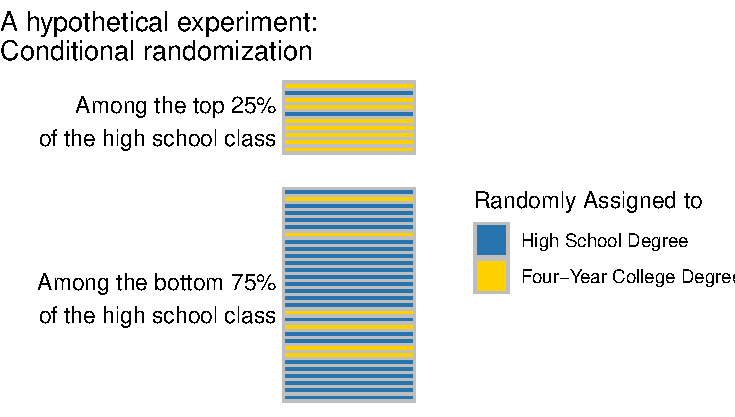
\includegraphics[width = \textwidth]{figures/conditional_randomization} \\
Outcome: Employed at age 40

\end{frame}

\section{Nodes and Edges}

\begin{frame}[t]{Elements of a Directed Acyclic Graph (DAG)}

\begin{center}
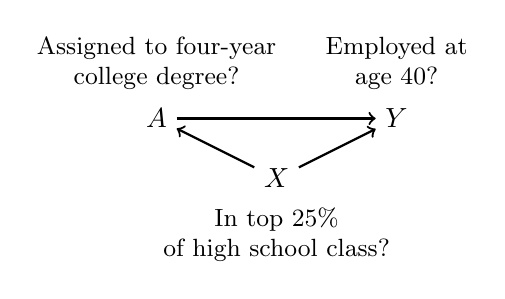
\begin{tikzpicture}[x = .3in, y = .3in]
    \node at (-3,0) {};
    \node at (3,0) {};
    \node (x) at (0,-1) {$X$};
    \node (a) at (-2,0) {$A$};
    \node (y) at (2,0) {$Y$};
    \draw[->, thick] (x) -- (a);
    \draw[->, thick] (a) -- (y);
    \draw[->, thick] (x) -- (y);
        % Labels
    \node[anchor = north, font = \small, align = center] at (x.south) {In top 25\%\\of high school class?};
    \node[anchor = south, font = \small, align = center] at (a.north) {Assigned to four-year\\college degree?};
    \node[anchor = south, font = \small, align = center] at (y.north) {Employed at\\age 40?};
  \end{tikzpicture}
\end{center}
  
  \begin{itemize}
  \item \textbf{Nodes} ($X,A,Y$) are random variables
  \item \textbf{Edges} ($\rightarrow$) are causal relationships.
  \begin{itemize}
  \item $X$ has a causal effect on $A$
  \item $X$ has a causal effect on $Y$
  \item $A$ has a causal effect on $Y$
  \end{itemize}
  \end{itemize}
  
\end{frame}

\begin{frame}[t]{Elements of a Directed Acyclic Graph (DAG)}

\begin{center}
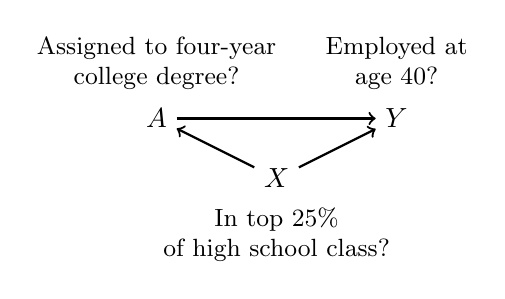
\begin{tikzpicture}[x = .3in, y = .3in]
    \node at (-3,0) {};
    \node at (3,0) {};
    \node (x) at (0,-1) {$X$};
    \node (a) at (-2,0) {$A$};
    \node (y) at (2,0) {$Y$};
    \draw[->, thick] (x) -- (a);
    \draw[->, thick] (a) -- (y);
    \draw[->, thick] (x) -- (y);
        % Labels
    \node[anchor = north, font = \small, align = center] at (x.south) {In top 25\%\\of high school class?};
    \node[anchor = south, font = \small, align = center] at (a.north) {Assigned to four-year\\college degree?};
    \node[anchor = south, font = \small, align = center] at (y.north) {Employed at\\age 40?};
  \end{tikzpicture}
\end{center}

A \textbf{path} is a sequence of edges connecting two nodes. \vskip .1in \pause
Between $A$ and $Y$, what are the two paths? \pause
\begin{itemize}
\item $A\rightarrow Y$
\item $A\leftarrow X \rightarrow Y$
\end{itemize}

\end{frame}

\section{Causal Paths}

\begin{frame}{Causal path: A path with arrows pointing one way}{$\bullet\rightarrow\bullet\rightarrow\bullet$} \pause

\begin{center}
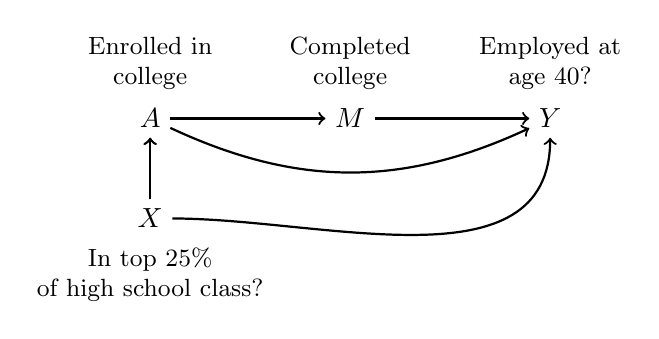
\begin{tikzpicture}[x = .5in, y = .5in]
    \node (x) at (-2,-1) {$X$};
    \node (a) at (-2,0) {$A$};
    \node (m) at (0,0) {$M$};
    \node (y) at (2,0) {$Y$};
    \draw[->, thick] (x) -- (a);
    \draw[->, thick] (a) to[bend right = 25] (y);
    \draw[->, thick] (a) -- (m);
    \draw[->, thick] (m) -- (y);
    \draw[->, thick] (x) -- (a);
    \draw[->, thick] (x) to[out = 0, in = 270] (y);
        % Labels
    \node[anchor = north, font = \small, align = center] at (x.south) {In top 25\%\\of high school class?};
    \node[anchor = south, font = \small, align = center] at (a.north) {Enrolled in\\college};
    \node[anchor = south, font = \small, align = center] at (m.north) {Completed\\college};
    \node[anchor = south, font = \small, align = center] at (y.north) {Employed at\\age 40?};
  \end{tikzpicture}
\end{center}
\pause
What three paths connect $A$ and $Y$? \\
Which two are causal paths? \vskip .1in
\pause
\begin{tabular}{ll}
$A\rightarrow Y$ & \only<5->{causal path} \\
$A\rightarrow M \rightarrow Y$ & \only<6->{causal path} \\
$A\leftarrow X \rightarrow Y$ & \only<7->{not a causal path}
\end{tabular}

\end{frame}

\begin{frame}[t]{Causal path: Marginal dependence}{$\bullet\rightarrow\bullet\rightarrow\bullet$} \vskip .2in

A causal path $A\rightarrow\cdots\rightarrow B$ will make the variables $A$ and $B$ statistically dependent \vskip .2in

Example:
$$(\text{visits grocery store}) \rightarrow (\text{buys ice cream}) \rightarrow (\text{eats ice cream})$$ \vskip .2in \pause

What if we condition:\\filter to those with (buys ice cream = \texttt{FALSE})?

\end{frame}

\begin{frame}[t]{Causal path: Conditional independence}{$\bullet\rightarrow\bullet\rightarrow\bullet$} \vskip .2in

A causal path $A\rightarrow\cdots\rightarrow B$ will not make the variables $A$ and $B$ statistically dependent if we condition on a variable along the path \vskip .2in

Example:
$$(\text{visits grocery store}) \rightarrow \boxed{(\text{buys ice cream})} \rightarrow (\text{eats ice cream})$$ \pause

Among people who didn't buy ice cream today,\\
those who went to the store and didn't\\
are equally likely to be eating ice cream. \vskip .2in \pause
Conditioning on (buys ice cream = \texttt{FALSE}) \textbf{blocks} this path.

\end{frame}

\section{Forks}

\begin{frame}[t]{Fork structure}{$\bullet\leftarrow\bullet\rightarrow\bullet$}

A sequence of edges within a path in which two variables are both caused by a third variable: $A\leftarrow C \rightarrow B$ \pause \vskip .1in

In our initial graph, what path contains a fork structure?

\begin{center}
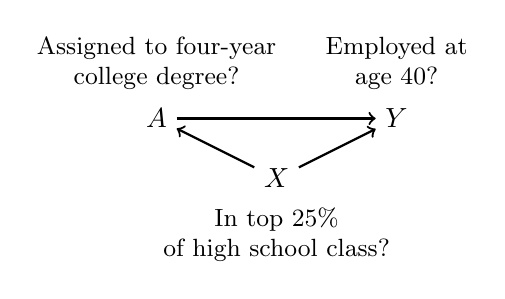
\begin{tikzpicture}[x = .3in, y = .3in]
    \node at (-3,0) {};
    \node at (3,0) {};
    \node (x) at (0,-1) {$X$};
    \node (a) at (-2,0) {$A$};
    \node (y) at (2,0) {$Y$};
    \draw[->, thick] (x) -- (a);
    \draw[->, thick] (a) -- (y);
    \draw[->, thick] (x) -- (y);
        % Labels
    \node[anchor = north, font = \small, align = center] at (x.south) {In top 25\%\\of high school class?};
    \node[anchor = south, font = \small, align = center] at (a.north) {Assigned to four-year\\college degree?};
    \node[anchor = south, font = \small, align = center] at (y.north) {Employed at\\age 40?};
  \end{tikzpicture}
\end{center}

Recall that there are two paths:
\begin{enumerate}
\item $A\rightarrow Y$
\item $A\leftarrow X \rightarrow Y$ \onslide<3->{(this path contains a fork structure)}
\end{enumerate}

\end{frame}

\begin{frame}[t]{Fork structure: Marginal dependence}{$\bullet\leftarrow\bullet\rightarrow\bullet$}

A fork structure $A\leftarrow C \rightarrow B$ will make $A$ and $B$ statistically dependent (because $C$ causes both). \vskip .1in

Example:
$$(\text{completed college}) \leftarrow (\text{top 25\% of high school})\rightarrow (\text{employed at 40})$$

\end{frame}

\begin{frame}[t]{Fork structure: Marginal dependence}{$\bullet\leftarrow\bullet\rightarrow\bullet$}

A fork structure $A\leftarrow C \rightarrow B$ will make $A$ and $B$ statistically dependent (because $C$ causes both). \vskip .1in

Example:
$$(\text{lifeguard rescues}) \leftarrow (\text{temperature})\rightarrow (\text{ice cream sales})$$ \pause

On days with many lifeguard rescues,\\there are also many ice cream sales.\\Warm temperature causes both. \vskip .2in \pause
What if we look only at days with a given temperature?

\end{frame}

\begin{frame}{Fork structure: Conditional independence}{$\bullet\leftarrow\bullet\rightarrow\bullet$}

A fork structure $A\leftarrow \boxed{C} \rightarrow B$ does not make $A$ and $B$ statistically dependent if we condition on $C$. \vskip .1in

Example:
$$(\text{lifeguard rescues}) \leftarrow \boxed{(\text{temperature})} \rightarrow (\text{ice cream sales})$$
Among days with a given temperature,\\lifeguard rescues and ice cream sales are unrelated. \vskip .2in
Conditioning on (temperature) blocks this path.

\end{frame}

\section{Colliders}

\begin{frame}{Collider structure}{$\bullet\rightarrow\bullet\leftarrow\bullet$}

A sequence of edges within a path in which two variables both cause a third variable: $A\rightarrow C \leftarrow B$ \pause \vskip .1in
Example:
\begin{itemize}
\item sprinklers on a timer
\item rain on random days
\item either one can make the grass wet
\end{itemize}

$$
(\text{sprinklers on}) \rightarrow (\text{grass wet}) \leftarrow (\text{raining})
$$ \pause
Are (sprinklers on) and (raining) statistically related?

\end{frame}

\begin{frame}{Collider structure: Marginal independence}{$\bullet\rightarrow\bullet\leftarrow\bullet$}

In a collider structure $A\rightarrow C \leftarrow B$,\\
$A$ and $B$ are marginally independent.
$$
(\text{sprinklers on}) \rightarrow (\text{grass wet}) \leftarrow (\text{raining})
$$
Knowing (sprinklers on = \texttt{TRUE}) tells me nothing about whether (raining = \texttt{TRUE}) \vskip .2in \pause

What if I condition: look only at days when the grass is wet?

\end{frame}

\begin{frame}{Collider structure: Conditional dependence}{$\bullet\rightarrow\bullet\leftarrow\bullet$}

$$
(\text{sprinklers on}) \rightarrow \boxed{(\text{grass wet})} \leftarrow (\text{raining})
$$ \vskip .2in \pause
Among days when (grass wet = \texttt{TRUE}),\\
if (sprinklers on = \texttt{FALSE})\\
then it must be (raining = \texttt{TRUE}) \vskip .1in
(grass had to get wet somehow!) \vskip .2in \pause

In a collider structure $A\rightarrow \boxed{C} \leftarrow B$,\\
$A$ and $B$ are conditionally dependent.

\end{frame}

\begin{frame}{Review: Three structures}

\begin{tabular}{llll}
& & $A$ and $B$ & $A$ and $B$ \\
& & marginally & conditionally \\
Name & Structure & dependent? & dependent given $C$? \\
\hline
Causal path & $A\rightarrow C \rightarrow B$ & Yes & No \\
Fork & $A\leftarrow C \rightarrow B$ & Yes & No \\
Collider & $A \rightarrow C \leftarrow B$ & No & Yes \\
\hline
\end{tabular}

\end{frame}

\section{Blocked Paths}

\begin{frame}[t]{A path can involve forks, colliders, and causal paths}

\begin{footnotesize}
$$
(\text{timer displays clock}) \leftarrow (\text{timer works}) \rightarrow (\text{sprinklers on}) \rightarrow (\text{grass wet}) \leftarrow (\text{raining})
$$
\end{footnotesize} \pause

(timer displays clock) is statistically related to which variables? \vskip .05in

\begin{tabular}{ll}
timer works & \onslide<3->{yes} \\
sprinklers on & \onslide<4->{yes} \\
grass wet & \onslide<5->{yes} \\
raining & \onslide<6->{no} \\
\end{tabular} \vskip .2in

\onslide<7->{We just learned: One collider can block an entire path}

\end{frame}

\begin{frame}[t]{A path can involve forks, colliders, and causal paths}

\begin{footnotesize}
$$
(\text{timer displays clock}) \leftarrow (\text{timer works}) \rightarrow \boxed{(\text{sprinklers on})} \rightarrow (\text{grass wet}) \leftarrow (\text{raining})
$$
\end{footnotesize} \pause

(timer displays clock) is statistically related to which variables? \vskip .05in

\begin{tabular}{ll}
timer works & \onslide<3->{yes} \\
grass wet & \onslide<4->{no} \\
raining & \onslide<5->{no} \\
\end{tabular} \vskip .2in

\onslide<6->{We just learned: One conditioned non-collider can block an entire path}

\end{frame}

\begin{frame}{Rules for whether paths are open or blocked}

\begin{itemize}
\item If a path contains an unconditioned collider, it is blocked
\item If a path contains a conditioned non-collider, it is blocked
\item Otherwise, the path is open
\end{itemize} \vskip .1in

Open paths create statistical dependence.\\Blocked paths do not.

\end{frame}

\section{Statistical Dependence}

\begin{frame}{Determining statistical dependence: A procedure}

How do you know if two nodes (e.g., $A$ and $B$ are dependent? \pause
\begin{center}
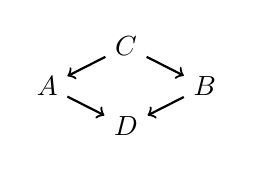
\begin{tikzpicture}[y = .2in]
\node (a) at (0,0) {$A$};
\node (b) at (2,0) {$B$};
\node (c) at (1,1) {$C$};
\node (d) at (1,-1) {$D$};
\draw[->, thick] (c) -- (a);
\draw[->, thick] (c) -- (b);
\draw[->, thick] (a) -- (d);
\draw[->, thick] (b) -- (d);
\end{tikzpicture}
\end{center} \pause
\begin{enumerate}
\item List all paths between the two nodes
\begin{itemize}
\item $A\leftarrow C \rightarrow B$
\item $A\rightarrow D \leftarrow B$
\end{itemize} \pause
\item Cross out any blocked paths that are blocked
\begin{itemize}
\item $A\leftarrow C \rightarrow B$
\item \st{$A\rightarrow D \leftarrow B$}
\end{itemize} \pause
\item If any paths remain, the two nodes are dependent
\begin{itemize}
\item Dependent!
\end{itemize}
\end{enumerate}

\end{frame}

% BUILDING UP EXAMPLE

\begin{frame}[t]{Determining statistical dependence: A procedure}{1. List all paths. 2. Cross out blocked paths. 3. Dependent if any paths remain.} \pause
\begin{center}
  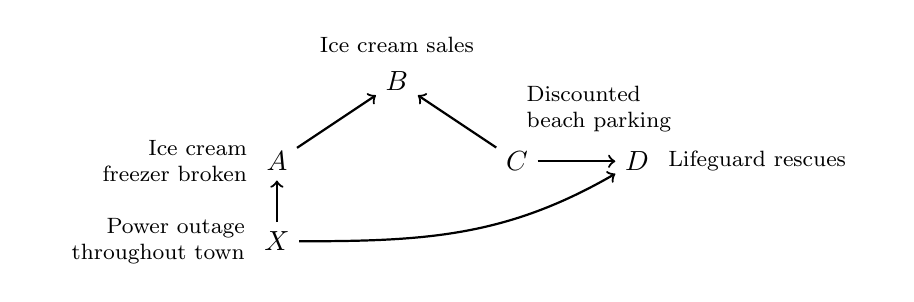
\begin{tikzpicture}[x = .6in, y = .4in]
  \node at (-2,0) {};
  \node at (5,0) {};
  \node (x) at (0,-1) {$X$};
  \node[anchor = east, font = \footnotesize, align = right] at (x.west) {Power outage\\throughout town};
  \pause
  \node (a) at (0,0) {$A$};
  \node[anchor = east, font = \footnotesize, align = right] at (a.west) {Ice cream\\freezer broken};
  \draw[->, thick] (x) -- (a);
  \pause
  \node (b) at (1,1) {$B$};
  \node[anchor = south, font = \footnotesize, align = right] at (b.north) {Ice cream sales};
  \draw[->, thick] (a) -- (b);
  \pause
  \node (c) at (2,0) {$C$};
  \node[anchor = south west, font = \footnotesize, align = left] at (c.north) {Discounted\\beach parking};
  \draw[->, thick] (c) -- (b);
  \pause
  \node (d) at (3,0) {$D$};
  \node[anchor = west, font = \footnotesize, align = right] at (d.east) {Lifeguard rescues};
  \draw[->, thick] (c) -- (d);
  \pause
  \draw[->, thick] (x) to[out = 0, in = 210] (d);
  \end{tikzpicture}
\end{center}
\end{frame}

% MARGINAL A AND C
\begin{frame}[t]{Determining statistical dependence: A procedure}{1. List all paths. 2. Cross out blocked paths. 3. Dependent if any paths remain.}
\begin{center}
  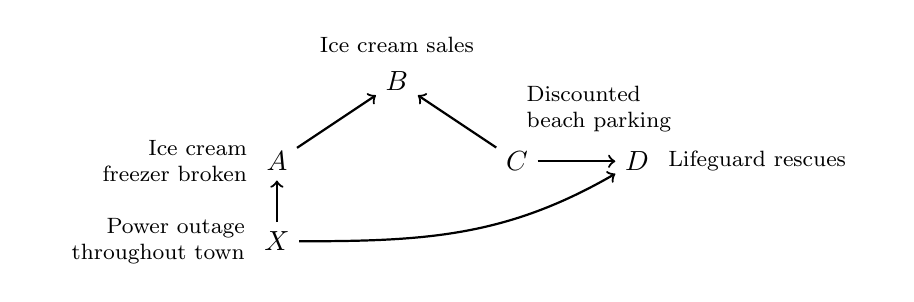
\begin{tikzpicture}[x = .6in, y = .4in]
  \node at (-2,0) {};
  \node at (5,0) {};
  \node (x) at (0,-1) {$X$};
  \node (a) at (0,0) {$A$};
  \node (b) at (1,1) {$B$};
  \node (c) at (2,0) {$C$};
  \node (d) at (3,0) {$D$};
  \draw[->, thick] (a) -- (b);
  \draw[->, thick] (c) -- (b);
  \draw[->, thick] (c) -- (d);
  \draw[->, thick] (x) -- (a);
  \draw[->, thick] (x) to[out = 0, in = 210] (d);
  \node[anchor = east, font = \footnotesize, align = right] at (a.west) {Ice cream\\freezer broken};
  \node[anchor = east, font = \footnotesize, align = right] at (x.west) {Power outage\\throughout town};
  \node[anchor = south, font = \footnotesize, align = right] at (b.north) {Ice cream sales};
  \node[anchor = south west, font = \footnotesize, align = left] at (c.north) {Discounted\\beach parking};
  \node[anchor = west, font = \footnotesize, align = right] at (d.east) {Lifeguard rescues};
  \end{tikzpicture}
\end{center}
Are $A$ and $C$ statistically independent or dependent?
\pause
\begin{itemize}
\item \only<3->{\st}{$A\rightarrow B \leftarrow C$}
\item \only<4->{\st}{$A\leftarrow X \rightarrow D \leftarrow C$}
\end{itemize}
\only<5>{No unblocked paths. Independent!}
\end{frame}

% MARGINAL A AND D
\begin{frame}[t]{Determining statistical dependence: A procedure}{1. List all paths. 2. Cross out blocked paths. 3. Dependent if any paths remain.}
\begin{center}
  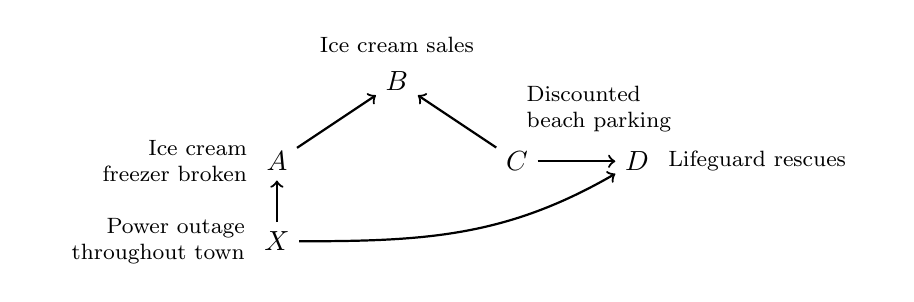
\begin{tikzpicture}[x = .6in, y = .4in]
  \node at (-2,0) {};
  \node at (5,0) {};
  \node (x) at (0,-1) {$X$};
  \node (a) at (0,0) {$A$};
  \node (b) at (1,1) {$B$};
  \node (c) at (2,0) {$C$};
  \node (d) at (3,0) {$D$};
  \draw[->, thick] (a) -- (b);
  \draw[->, thick] (c) -- (b);
  \draw[->, thick] (c) -- (d);
  \draw[->, thick] (x) -- (a);
  \draw[->, thick] (x) to[out = 0, in = 210] (d);
  \node[anchor = east, font = \footnotesize, align = right] at (a.west) {Ice cream\\freezer broken};
  \node[anchor = east, font = \footnotesize, align = right] at (x.west) {Power outage\\throughout town};
  \node[anchor = south, font = \footnotesize, align = right] at (b.north) {Ice cream sales};
  \node[anchor = south west, font = \footnotesize, align = left] at (c.north) {Discounted\\beach parking};
  \node[anchor = west, font = \footnotesize, align = right] at (d.east) {Lifeguard rescues};
  \end{tikzpicture}
\end{center}
Are $A$ and $D$ statistically independent or dependent? \pause
\begin{itemize}
\item \only<3->{\st}{$A\rightarrow B \leftarrow C \rightarrow D$}
\item $A\leftarrow X \rightarrow D$
\end{itemize}
\only<4>{A path remains unblocked. Dependent!}

\end{frame}

% CONDITIONAL

%\section{Conditional Dependence}

\begin{frame}

\huge
Practice with \textbf{conditional} dependence\\
(holding something constant)

\end{frame}

\begin{frame}[t]{Determining statistical dependence: A procedure}{1. List all paths. 2. Cross out blocked paths. 3. Dependent if any paths remain.}
\begin{center}
  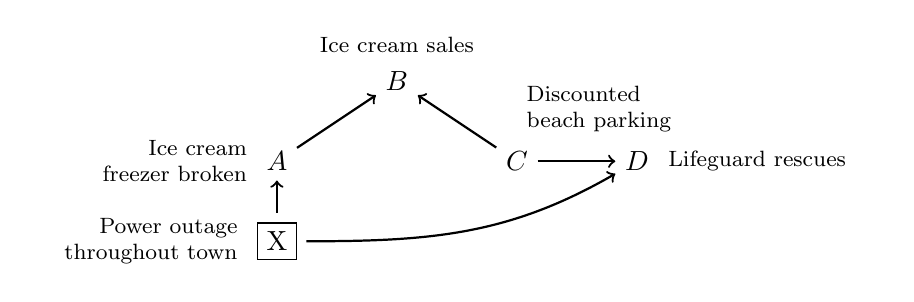
\begin{tikzpicture}[x = .6in, y = .4in]
  \node at (-2,0) {};
  \node at (5,0) {};
  \node (x) at (0,-1) {\boxed{$X$}};
  \node (a) at (0,0) {$A$};
  \node (b) at (1,1) {$B$};
  \node (c) at (2,0) {$C$};
  \node (d) at (3,0) {$D$};
  \draw[->, thick] (a) -- (b);
  \draw[->, thick] (c) -- (b);
  \draw[->, thick] (c) -- (d);
  \draw[->, thick] (x) -- (a);
  \draw[->, thick] (x) to[out = 0, in = 210] (d);
  \node[anchor = east, font = \footnotesize, align = right] at (a.west) {Ice cream\\freezer broken};
  \node[anchor = east, font = \footnotesize, align = right] at (x.west) {Power outage\\throughout town};
  \node[anchor = south, font = \footnotesize, align = right] at (b.north) {Ice cream sales};
  \node[anchor = south west, font = \footnotesize, align = left] at (c.north) {Discounted\\beach parking};
  \node[anchor = west, font = \footnotesize, align = right] at (d.east) {Lifeguard rescues};
  \end{tikzpicture}
\end{center}
Practice: Are $A$ and $D$ statistically independent or dependent, conditional on $X = \texttt{FALSE}$?
\pause
  \begin{itemize}
\item \only<3->{\st}{$A\rightarrow B \leftarrow C \rightarrow D$}
\item \only<4->{\st}{$A\leftarrow \boxed{X} \rightarrow D$}
\end{itemize}
\only<5>{No unblocked paths. Independent!}
\end{frame}
  
\begin{frame}[t]{Determining statistical dependence: A procedure}{1. List all paths. 2. Cross out blocked paths. 3. Dependent if any paths remain.}
\begin{center}
  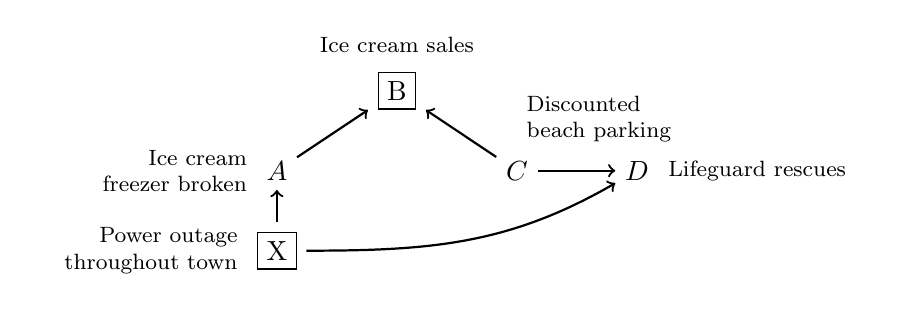
\begin{tikzpicture}[x = .6in, y = .4in]
  \node at (-2,0) {};
  \node at (5,0) {};
  \node (x) at (0,-1) {\boxed{$X$}};
  \node (a) at (0,0) {$A$};
  \node (b) at (1,1) {\boxed{$B$}};
  \node (c) at (2,0) {$C$};
  \node (d) at (3,0) {$D$};
  \draw[->, thick] (a) -- (b);
  \draw[->, thick] (c) -- (b);
  \draw[->, thick] (c) -- (d);
  \draw[->, thick] (x) -- (a);
  \draw[->, thick] (x) to[out = 0, in = 210] (d);
  \node[anchor = east, font = \footnotesize, align = right] at (a.west) {Ice cream\\freezer broken};
  \node[anchor = east, font = \footnotesize, align = right] at (x.west) {Power outage\\throughout town};
  \node[anchor = south, font = \footnotesize, align = right] at (b.north) {Ice cream sales};
  \node[anchor = south west, font = \footnotesize, align = left] at (c.north) {Discounted\\beach parking};
  \node[anchor = west, font = \footnotesize, align = right] at (d.east) {Lifeguard rescues};
  \end{tikzpicture}
\end{center}
Practice: Are $A$ and $D$ statistically independent or dependent, conditional on $X = \texttt{FALSE}$ and $B = \texttt{0}$?
\pause
  \begin{itemize}
\item $A\rightarrow \boxed{B} \leftarrow C \rightarrow D$
\item \only<3->{\st}{$A\leftarrow \boxed{X} \rightarrow D$}
\end{itemize}
\only<4>{A path remains. Dependent!}
\end{frame}

\section{Conditional Exchangeability}

\begin{frame}{DAGs and conditional exchangeability}

When studying the effect of $A$ on $Y$, conditional exchangeability holds if the only unblocked paths between $A$ and $Y$ are causal paths from $A$ to $Y$. \pause
\begin{itemize}
\item Why? Because then any association between $A$ and $Y$ must be due to the causal effect
\end{itemize} \pause
\begin{center}
  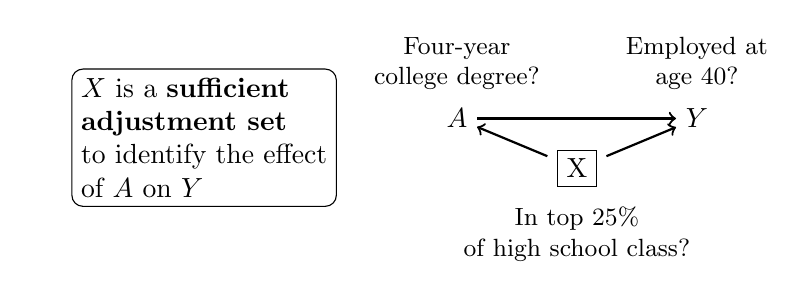
\begin{tikzpicture}[x = .3in, y = .25in]
    \node at (-9,0) {};
    \node at (3,0) {};
    \node (x) at (0,-1) {\boxed{$X$}};
    \node (a) at (-2,0) {$A$};
    \node (y) at (2,0) {$Y$};
    \draw[->, thick] (x) -- (a);
    \draw[->, thick] (a) -- (y);
    \draw[->, thick] (x) -- (y);
    % Labels
    \node[anchor = north, font = \small, align = center] at (x.south) {In top 25\%\\of high school class?};
    \node[anchor = south, font = \small, align = center] at (a.north) {Four-year\\college degree?};
    \node[anchor = south, font = \small, align = center] at (y.north) {Employed at\\age 40?};
    \node<5->[anchor = north east, align = left, draw, rounded corners] at (-4,1) {$X$ is a \textbf{sufficient}\\\textbf{adjustment set}\\to identify the effect\\of $A$ on $Y$};
  \end{tikzpicture}
  \end{center} \pause
\begin{itemize}
\item $A\rightarrow Y$
\item $A\leftarrow \boxed{X} \rightarrow Y$ (blocked by conditioning on $X$)
\end{itemize}

\end{frame}

\begin{frame}{DAGs and conditional exchangeability: Practice}
{1. List all paths. 2. Choose adjustment set. 3. Only causal paths remain unblocked.}

\begin{center}
  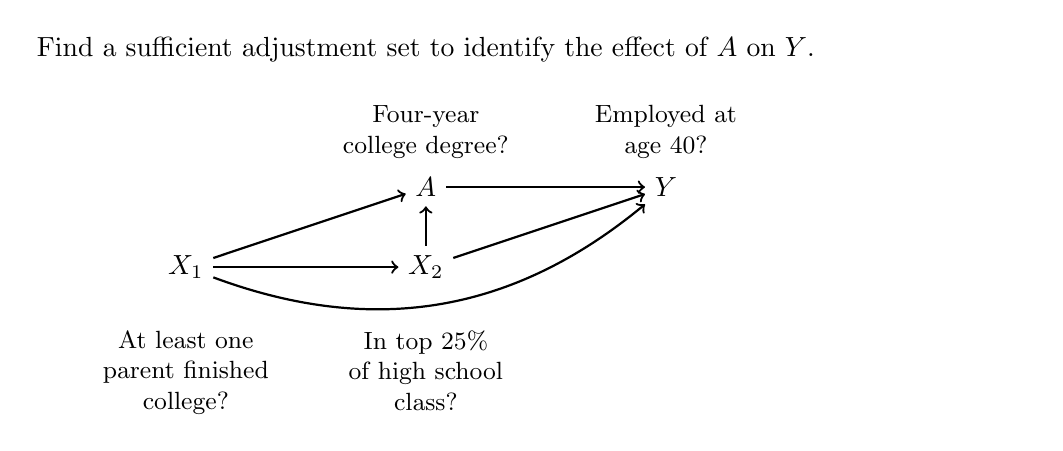
\begin{tikzpicture}[x = .6in, y = .4in]
  \node[anchor = north] at (-2,2) {Find a sufficient adjustment set to identify the effect of $A$ on $Y$.};
    \node at (-3,0) {};
    \node at (3,0) {};
    \node (x1) at (-4,-1) {$X_1$};
    \node (x2) at (-2,-1) {$X_2$};
    \node (a) at (-2,0) {$A$};
    \node (y) at (0,0) {$Y$};
    \draw[->, thick] (x1) -- (a);
    \draw[->, thick] (x1) to[bend right = 30] (y);
    \draw[->, thick] (x1) -- (x2);
    \draw[->, thick] (x2) -- (a);
    \draw[->, thick] (a) -- (y);
    \draw[->, thick] (x2) -- (y);
    % Labels
    \node[anchor = north, font = \small, align = center, outer sep = 12pt] at (x1.south) {At least one\\parent finished\\college?};
    \node[anchor = north, font = \small, align = center, outer sep = 12pt] at (x2.south) {In top 25\%\\of high school\\class?};
    \node[anchor = south, font = \small, align = center] at (a.north) {Four-year\\college degree?};
    \node[anchor = south, font = \small, align = center] at (y.north) {Employed at\\age 40?};
  \end{tikzpicture}
  \end{center} \pause

Paths: ($A\rightarrow Y$), ($A\leftarrow X_2\rightarrow Y$), ($A\leftarrow X_1\rightarrow Y$), ($A\leftarrow X_1\rightarrow X_2\rightarrow Y$),($A\leftarrow X_2\leftarrow X_1\rightarrow Y$) \\ \pause
Adjust for \{$X_1,X_2\}$

\end{frame}

\begin{frame}{How to draw a DAG}

\begin{enumerate}
\item Begin with treatment $A$ and outcome $Y$
\item Add any variable that affects both
\item Add any variable that affects any two variables in the DAG.
\end{enumerate}

Assumptions are about nodes and edges that you omit.

\end{frame}

\begin{frame}{Exercise: Draw a DAG}

Treatment is college degree. Outcome is employment at age 40.

\end{frame}

\goalsframe

\end{document}

